\documentclass[12pt,letterpaper]{article}
\usepackage{fullpage, times}
\usepackage{hyperref}
\usepackage{ctable}
\begin{document}
\title{Deploying and Sharing QSAR Models using Predictive Modeling Markup Language}
\author{Villu Ruusmann${}^{\dagger}$ and Rajarshi Guha${}^{\ddagger}$\\
${}^{\ddagger}$National Center for Advancing Translational Sciences\\ 9800 Medical Center Drive  Rockville, MD 20850 \\ \\
${}^{\dagger}$Your address }
\date{}
\maketitle
\begin{abstract}
  A nice abstract
\end{abstract}

\section{A Plethora of Predictive Models}
\label{sec:introduction}

Quantitative Structure-Activity Relationship (QSAR) models have become
ubiquitous in computational chemistry and cheminformatics, having been
built for a variety of endpoints including biological activities and
physical properties. As shown in Figure \ref{fig:count-qsar} the last
15 years has seen a significant increase in publications developing or
using QSAR models. While there has been much discussion (REFS) on the
prospective utility and validity of predictive QSAR models, a key
bottleneck to their assessment is the fact that they are not easily
obtainable. That is, the bulk of QSAR models are described in a
publication in terms of the descriptors (sometimes made available) and
the modeling method. While the implementation is noted, it is upon the
reader to actually obtain the descriptor values, obtain and set up the
modeling environment and then actually rebuild the model. In other
words, the actual model that was developed by the authors is, usually,
not available to be used directly. In a few cases, the model may be
built in a pipeline tool [REF], which alleviates this problem to some
extent. Furthermore, the model development workflow usually involves
multiple software tools, each one of a specific version. Without
access to the exact same version of these tools, a user cannot be
guaranteed to exactly reproduce the model that the authors
describe. The issue of reproducibility (of workflows and results) has
become increasingly important [REF Greg Landrum] in the computational
arena.

A number of workers have described infrastructure to deploy predictive
models. Some platforms such as Pipeline Pilot provide a easy to use
method to deploy a complete pipeline as a web page. However, this
approach does not allow one to share models with users who do not have
access to the software. Guha [REF] described a web based
infrastructure that allowed one to deploy serialized models developed
in R. This architecture allowed one to distribute the model via a web
page, allowing users to provide new input and retrieve
predictions. But by virtue of using serialized R models, it allowed
the user to directly work with the original model itself. An important
downside was that the model itself did not contain explicit references
to the descriptors that were required as input. 

Bioclipse

\subsection{Model reproducibility vs. Model reusability}

The main question: if you see a QSAR model in the literature, do you
want to analyze its mathematical properties, or do you want to apply
it to your dataset in order to see how it performs?

One of the principles of the scientific method is that the research
must be repeatable and reproducible. From the QSAR point of view there
are not much technical obstacles in the way. The biggest concern is
using proprietary algorithms and software.

Model reproducibility is about marking down the procedure by which
the model can be derived given the same input data. Theoretical methods
do not have random error component[?]. Thus, all deviations must be
explained by systematic errors, which could be related to choosing the
wrong algorithm, wrong parametrization etc.

Documenting the whole model training and validation process with the
help of electronic laboratory notebooks. Should include both human and
machine readable instructions of the process. The latter can be given 
in the form of an executable script (ie. when executed with appropriate
input data, produces the model and output data). Plenty of options to
choose from (open source):
\begin{itemize}
  \item knitr \url{http://yihui.name/knitr/}
  \item Sweave \url{https://www.stat.uni-muenchen.de/~leisch/Sweave/}
  \item Sage \url{http://www.sagemath.org/}
  \item IPython \url{http://ipython.org/}
\end{itemize}

The ONS approach is to use Wiki pages, which contain embedded R code
and plots. For example, see
\url{http://onschallenge.wikispaces.com/MeltingPointModel002}.

Most of the time, however, the reader in interested in the \emph{final
ending state} of the modeling workflow. That is, the mathematical 
relationship that has been properly validated and whose applicability 
domain has been sufficiently characterized.

Essentially, the representation of a model training process boils down
to representing the training algorithm. The most complete representation
is in application code such as R, Python, MATLAB etc.
The algorithm "works" by applying a finite list of well-defined 
instructions to the initial state. After applying each instruction the
system reaches another state. When the list of instructions has been
exhausted the system has reached its final ending state.
The representation of states is technically much more challenging than 
the representation of algorithms. A state may consist of different
parts. We are only interested in that part, which relates to the 
mathematical relationship. A state can be preserved by taking a snapshot
of the particular memory area. To make reading and writing more easier,
should be formalized as a data structure.

\subsection{Elements of a predictive solution}

A model represents a standalone mathematical relationship. Not very easy
to work with from the end user perspective. A model should be packaged
as a predictive solution, which has the following components:
\begin{itemize}
  \item Data schema. Specifies information about input and output fields.
  Data schema represents the "public interface" for the end user. 
  For example, data schema could communicate that a predictive solution
  consumes a single string-type input field that contains the SMILES 
  representation of a chemical structure, and produces two output fields - 
  a string-type field that contains the classification result (eg. the 
  predicted mechanism of toxic action) and a floating point-type field 
  that contains a class-specific regression result (eg. if the chemical
  structure was classified as a narcotic agent, the predicted pIGC50 
  value using the narcosis QSAR model).
  \item Data pre- and post-processing functions. Typically, the input
  fields that are listed in data schema cannot be directly fed to the 
  underlying matchematical relationship "as is". Could be related to 
  translating input from user representation to internal representation
  (eg. converting SMILES to CDK molecular graph to CDK descriptor value)
  or performing additional transformations on it (eg. normalization, 
  converting from natural scale to logaritmic scale etc.).Similarly,
  could derive secondary output fields based on the primary field. For
  example, calculating the probability of the predicted class or standard
  error of the predicted value.
  \item Data (work)flows. A predictive solution may encapsulate more
  than one model. The passage of data from one model to another happens
  inside the predictive solution. Two most common scenarious is model 
  aggregation, where the final prediction is calculated by applying an
  aggregation function over a list of interim predictions (eg. consensus
  modeling), and model chaining, where the output of earlier models
  becomes the input of subsequent models (eg. classification followed 
  by regression).
\end{itemize}

TODO: A figure of a chemistry-specific predictive solution.

\subsection{The lifecycle of a predictive solution}

A modeling workflow has two clearly distinguishable lifecycle phases:
\begin{enumerate}
  \item Training. Happens once in the very beginning. Handled by a data
  scientist. Typically in desktop environment. 
  \item Deployment.Happens many times. Handled by plurality of IT 
  roles/personnel. Typically in server-side environment, different 
  platforms/runtimes. 
\end{enumerate}

The training is handled by a scientist. Involves analysing the
"fundamental side" of the problem, choosing the right statistical 
algorithms for training and validation. Also, providing the mechanistic
interpretation of the results (white box models). The result is 
shared with peers using modern scientific communication means. Provided
that the result is actually useful, many people may want to deploy it
on their premises afterwards.

The deployment is an operational IT problem. Different organizations 
may prefer different platforms, data frameworks. Therefore, the trained
predictive solution should be maximally portable.

The portability can be best acieved by relying on open and popular
standards. To a lesser degree, if no standards have been established yet,
could rely on open and popular tools. For example, CDK is not formally
backed by a standard, but it is generally very easy to use and integrate
with different chemistry products, because its source code can be obtained
and modified easily.

Overall, moving models from training phase to deployment phase is a
major hurdle in practical data science. It is estimated that in corporate
environments the average length of a modeling iteration may be as long
as 16-24 months [private conversation, public ref?]. All approaches that
can reduce this timespan and associated costs could provide significant
business value.

\subsection{Serializing Models}
\label{sec:serializing-models}

A key step in sharing predictive models is serialization. That is,
converting the internal representation of the model developed in some
environment (R, Weka, Matlab, Mathematica etc) to a disk file (usually
a sequence of bytes). Not all deployment approaches require this step
- usually platforms that host the deployment and development
mechanisms (e.g., Pipeline Pilot, R using Shiny [REF]). But in general, for one to share a
model, it must be serialized and the serialized form is exchanged.

Most model development platforms support binary serialization
schemes. For example, R can save models in the RData format [REF]
which is binary and can only be read by the R platform (though since
it is Open Source, one could read/write such files using custom
code). XXX What about Matlab? XXX Java objects (say from Weka) can
be serialized using the Java Object Protocol [REF http://docs.oracle.com/javase/7/docs/technotes/guides/serialization/]

In contrast to binary serialization formats, the Predictive Modeling
Markup Language is a plain text XML format that is designed to fully
describe the model. Importantly, with appropriate software a PMML
document can be used to reconstruct the model, including any data
preprocessing steps (scaling, normalization) as well as generate input
descriptors if appropriately specified. A number of software tools are
capable of reading and writing PMML documents including SAS, SPSS,
TIBCO and KNIME, whereas others such as R can produce PMML documents
and WEKA which can consume PMML documents.


\ctable[cap={}, caption={Growth in number of Pubmed articles that use the term QSAR.},
label={fig:count-qsar},figure,botcap]
{c}
{}
{
  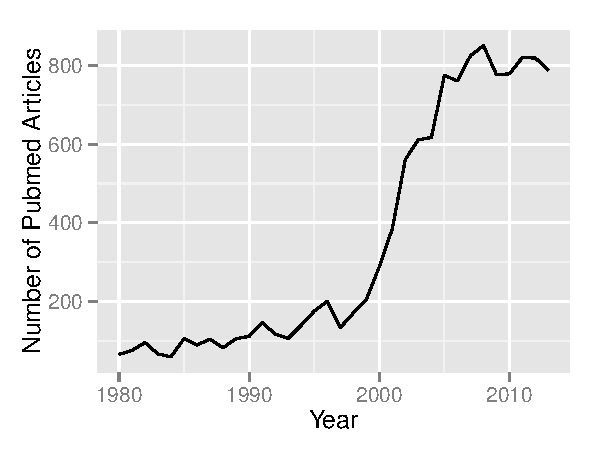
\includegraphics{img/count-qsar}
}

\section{Methods}
\label{sec:methods}

\subsection{Model Development}
\label{sec:model-development}

For this study we developed models in R 3.1 [REF] with descriptors
generated using the CDK [REF] via the rcdk [REF] package. As exemplars
we considered two datasets. XXX Describe the datasets.

Next we developed a linear regression (or classification) and random
forest  model  for each dataset. Using the pmml package [REF] we
serialized the models to PMML.

\subsection{Model Deployment}
\label{sec:model-deployment}


\section{Discussion}
\label{sec:discussion}

\subsection{PMML Supports Open Science}
\label{sec:pmml-supports-open}





\end{document}
